\documentclass[11pt]{report}
\usepackage[margin=2cm]{geometry}
\usepackage{graphicx}
\usepackage{float}
\usepackage{times}

\newcommand{\Gap}{\texorpdfstring{\hfill}{}}
\newcommand{\Rec}{\texorpdfstring{{\small\emph{\color{blue}{\fbox{High Leverage}}}}}{}}
\newcommand{\HighRisk}{\texorpdfstring{{\small\emph{\color{orange}{\fbox{Uncertain Impact}}}}}{}}
\newcommand{\Longterm}{\texorpdfstring{{\small\emph{\color{OliveGreen}{\fbox{Long-term}}}}}{}}

\usepackage[dvipsnames]{xcolor}

\begin{document}

\section{Societal Impacts\texorpdfstring{\hfill\textit{by Kris Sankaran}}{}}
\label{sec:societal-impacts}

Changes in the atmosphere have impacts on the ground.
The expected societal impacts of climate change include prolonged ecological and
socioeconomic stresses as well as brief, but severe, societal disruptions. For example, impacts could include both gradual decreases in crop yield and localized food shortages.
If we can anticipate climate impacts well enough, then we can prepare for
them by asking:

\begin{itemize}
\item How do we reduce vulnerability to climate impacts?
\item How do we support rapid recovery from climate-induced disruptions?
\end{itemize}

A wide variety of strategies have been put forward, from robust power grids to
food shortage prediction (Fig.~\ref{fig:society}), and while this is good news for society, it can be
overwhelming for an ML practitioner hoping to contribute. Fortunately, a few
critical needs tend to recur across strategies -- it is by meeting
these needs that ML has the greatest potential to support societal adaptation
\cite{ford2016opinion, quinn2014computational, kelling2018computational}.
From a high level, these involve
\begin{itemize}
\item Sounding alarms: Identifying and prioritizing the areas of highest risk, by using evidence of risk from historical data.
\item Providing annotation: Extracting actionable information or labels from unstructured raw data.
\item Promoting exchange: Making it easier to share resources and information to pool and reduce risk.
\end{itemize}

These unifying threads will appear repeatedly in the sections below, where we review strategies to help ecosystems, infrastructure, and societies adapt to climate change, and explain how ML supports each strategy (Fig.~\ref{fig:society}).
\begin{figure}[hppt]
    \centering
    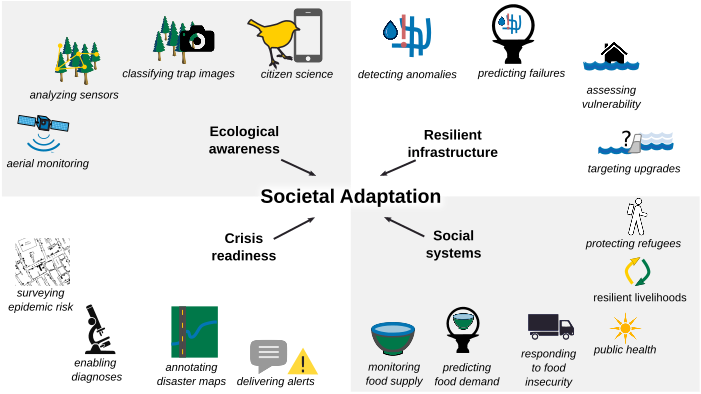
\includegraphics[width=\textwidth]{figures/societal-adaptation.png}
    \caption{Selected strategies to accelerate societal adaptation to climate change using machine learning.}
    \label{fig:society}
\end{figure}

We note that the projects involved vary in scale from local to global, from infrastructure upgrades
and crisis preparedness planning to international ecosystem monitoring and
disease surveillance. Hence, we anticipate valuable contributions by
researchers who have the flexibility to formulate experimental
approaches, by industrial engineers and entrepreneurs who have the expertise to
translate prototypes into wide-reaching systems, and by civil servants who lead
many existing climate adaptation efforts.

\subsection{Ecology}
\label{subsub:ecology}

Changes in climate are increasingly affecting the distribution and composition of ecosystems. This has profound implications for global biodiversity, as well as agriculture, disease, and natural resources such as wood and fish.
ML can  help by supporting efforts to monitor ecosystems and biodiversity.

\paragraph*{Monitoring ecosystems}\Gap\textbf{\Rec}\mbox{}\\ To preserve
ecosystems, it is important to know which are most at risk. This has
traditionally been done via manual, on-the-ground observation, but the process
can be accelerated by annotation of remote sensing data
\cite{potter2008terrestrial,boriah2008land,malkin2018label,bragilevsky2017deep} (see also \S\ref{sec:emissions-detection}). For example,
tree cover can be automatically extracted from aerial imagery to characterize
deforestation \cite{mcdowell2015global, huynh2018annotation}. At the scale of
regions or biomes, analysis of large-scale simulations can illuminate the
evolution of ecosystems across potential climate futures
\cite{klausmeyer2009climate, feng2018improving}. A more direct source of data is
offered by environmental sensor networks, made from densely packed but low-cost
devices \cite{hart2006environmental, dietterich2009machine, hut2012tahmo}. To
monitor ocean ecosystems, marine robots are useful, because they can be used to
survey large areas on demand \cite{griffiths1998towards, dunbabin2012robots}.

For a system to have the most real-world impact, regardless of the underlying
data source, it is necessary to ``personalize'' predictions across a range of
ecosystems. A model trained on the Sahara would almost certainly fail if
deployed in the Amazon. Hence, these applications may motivate ML researchers
interested in heterogeneity, data collection, transfer learning, and rapid
generalization. In sensor networks, individual nodes fail frequently, but are
redundant by design -- this is an opportunity for research into anomaly
detection and missing data imputation \cite{dereszynski2012probabilistic,hill2010anomaly}. In marine robotics, improved techniques for sampling regions
to explore and automatic summarization of expedition results would both provide
value \cite{das2015data, flaspohler2017feature}. Finally, beyond aiding
adaptation by prioritizing at-risk environments, the design of effective methods
for ecosystem monitoring will support the basic science necessary to shape
adaptation in the long-run \cite{faghmous2014big,gomes2009computational,marotzke2017climate}.

\paragraph*{Monitoring biodiversity }\Gap\textbf{\Rec}\mbox{}\\
Accurate estimates of species populations are the foundation on which conservation efforts are built. Camera traps and aerial imagery have increased the richness and coverage of sampling efforts. ML can help infer biodiversity counts from image-based sensors.
For instance, camera traps take photos automatically whenever a motion sensor is activated -- computer vision can be used to classify the species that pass by, supporting a real-time, less labor-intensive species count \cite{zamba, beery2019synthetic, norouzzadeh2018automatically}. It is also possible to use aerial imagery to estimate the size of large herds \cite{van2014nature} or count birds \cite{ghioca2008assessing}. In underwater ecosystems, ML has been used to identify plankton automatically from underwater cameras \cite{faillettaz2016imperfect} and to infer fish populations from the structure of coral reefs \cite{young2018convolutional}.

Citizen science can also enable dataset collection at a scale impossible in individual studies \cite{sullivan2009ebird, plantsnap, branchini2015using, menon2016animal}. For example, by leveraging public enthusiasm for birdwatching, eBird has logged more than 140 million observations \cite{sullivan2009ebird}, which have been used for population and migration studies \cite{kelly2016novel}. Computer vision algorithms that can classify species from photographs have furthered such citizen science efforts by making identifications easier and more accurate \cite{van2015building, ralls2018systems}, though these face challenges such as class imbalances in training data \cite{van2017devil}. Work with citizen science data poses the additional challenge that researchers have no control over where samples come from. To incentivize observations from undersampled regions, mechanisms from game theory can be applied \cite{xue2016avicaching}, and even when sampling biases persist, estimates of dataset shift can minimize their influence \cite{chen2018bias}.

Monitoring biodiversity may be paired with interventions to protect rare species or control invasive pests. Machine learning is providing new solutions to assess the impact of ecological interventions \cite{rana2018machine, albers2018role, lydakiscomputing} and prevent poaching \cite{xue2016avicaching}.

\subsection{Infrastructure} \label{subsub:infrastructure}

Physical infrastructure is so tightly woven into the fabric of everyday life -- like the buildings we inhabit and lights we switch on -- that it is easy to forget that it exists (see \S\ref{sec:buildings-cities}). The fact that something so basic will have to be rethought in order to adapt to climate change can be unsettling, but viewed differently, the sheer necessity of radical redesign can inspire creative thinking.

We first consider the impacts of climate change on the built environment. Shifts in weather patterns are likely to put infrastructure under more persistent stress. Heat and wind damage roads, buildings, and power lines. Rising water tables near the coast will lead to faults in pipelines. Urban heat islands will be exacerbated and it is likely that there will be an increased risk of flooding caused by heavy rain or coastal inundations, resulting in property damage and traffic blockages\cite{Pachauri2014}.

A clear target is construction of physical defenses -- for example, ``climate proofing'' cities with new coastal embankments and increased storm drainage capacity.  However, focusing solely on defending existing structures can stifle proactive thinking about urban and social development -- for example, floating buildings are being tested in Rotterdam -- and one may alternatively consider resilience and recovery more broadly \cite{pelling2010adaptation, shi2016roadmap}. From this more general perspective  of improving social processes, ML can support two types of activities: Design and maintenance.

\paragraph*{Designing infrastructure}\Gap\textbf{\Longterm}\mbox{}\\ How can infrastructure be (re)designed to dampen climate impacts?
In road networks, it is possible to incorporate flood hazard and traffic
information in order to uncover vulnerable stretches of road, especially those with few
alternative routes \cite{gupta2018infrastructure}. If traffic data are not
directly available, it is possible to construct  proxies from mobile
phone usage and city-wide CCTV streams -- these are promising in rapidly developing
urban centers \cite{frias2012estimation, jain2012road}. Beyond drawing from
flood hazard maps, it is possible to use data from real-world flooding events
\cite{pastor2014flooding}, and to send localized predictions to those at risk 
\cite{wiesel2018ml}.
For electrical, water, and waste collection networks, the same
principle can guide investments in resilience -- using proxy or historical data
about disruptions to anticipate vulnerabilities 
\cite{oshri2018infrastructure, muharemi2019machine, nateghi2018multi, panteli2015grid}. 
Robust components can replace those at risk; for example, \emph{adaptive islands}, parts of an energy grid that continue to provide power even when disconnected from the network, 
prevent cascading outages in power distribution \cite{fang2012smart}.

Infrastructure is long-lived, but the future is uncertain, and planners must weigh immediate resource costs against future societal risks \cite{fletcher2019learning}. One area that urgently needs adaptation strategies is the consistent access to drinking water, which can be jeopardized by climate variability \cite{delpla2009impacts, unihe}. Investments in water infrastructure can be optimized; for example, a larger dam might cost more up front, but would have a larger storage capacity, giving a stronger buffer against drought. To delay immediate decisions, infrastructure can be upgraded in phases -- the technical challenge is to discover policies that minimize a combination of long-term resource and societal costs under plausible climate futures, with forecasts being updated as climates evolve \cite{quinn2017direct, giuliani2015curses, shen2017trans}.

\paragraph*{Maintaining infrastructure}\Gap\textbf{\Rec}\mbox{}\\ What types of systems can keep infrastructure functioning
well under increased stress? Two strategies for efficiently managing limited
maintenance resources are predictive maintenance and anomaly detection;
both can be applied to electrical, water, and transportation
infrastructure. In predictive maintenance, operations are prioritized according
to the predicted probability of a near-term breakdown \cite{rudin2012machine,
nguyen2018automatic, srivastava2018design, dragomir2009review}. For anomaly detection, failures are discovered as soon as
they occur, without having to wait for inspectors to show up, or complaints to
stream in \cite{baig2011use, difallah2013scalable}. 

The systems referenced here have required the manual curation of data streams,
structured and unstructured. The data are plentiful, just difficult to glue
together. Ideas from the missing data, multimodal data, and AutoML communities
have the potential to resolve some of these issues.

\subsection{Social systems}
\label{subsub:social_systems}

While less tangible, the social systems we construct are just as critical to the
smooth functioning of society as any physical infrastructure, and it is
important that they adapt to changing climate conditions. First, consider
what changes these systems may encounter. Decreases in crop yield, due to drought and other factors, will pose a threat to food
security, as already evidenced by long periods of drought in North America, West
Africa and East Asia \cite{ipcc_foodsec, dai2011drought}. More generally, communities
dependent on ecosystem resources will find their livelihoods at risk, and this
may result in mass migrations, as people seek out more supportive environments.

At first, these problems may seem beyond the reach of algorithmic thinking,
but investments in \textit{social} infrastructure can increase
resilience. ML can amplify the reach and effectiveness of this infrastructure. See also \S{\ref{sec:toolsforsociety}} for
perspective on how ML can support the function and analysis of complex
social environments.

\paragraph*{Food security}\Gap\textbf{\Rec}\mbox{}\\
Data can be used to monitor the risk of food insecurity in real time, to forecast
near-term shortages, and to identify areas at risk in the long-term, all of which
can guide interventions. For real-time and near-term systems, it is
possible to distill relevant signals from mobile phones, credit card
transactions, and social media data \cite{decuyper2014estimating,
pulse2015using, kim2017nowcasting}. These have emerged as low-cost, high-reach
alternatives to manual surveying. The idea is to train models that link these
large, but decontextualized, data with ground truth consumption or survey
information, collected on small representative samples. This process of 
developing proxies to link small, rich datasets with large, coarse ones 
can be viewed as a type of semi-supervised learning, and is fertile ground
for research.

For longer-term warnings, spatially localized crop yield predictions are needed.
These can be generated by aerial imagery or meteorological data (see \S\ref{sec:agriculture}), if they can be
linked with historical yield data \cite{Chakraborty2011, wang2018deep}. 
On the ground, it is possible to perform crop-disease
identification from plant photos -- this can alert communities to disease
outbreaks, and enhance the capacity of agricultural inspectors. For even
longer-run risk evaluation, it is possible to simulate crop yield via biological
and ecological models \cite{tebaldi2008towards,rosenzweig2014assessing,konduri_kumar_hoffman_bhatia_gouthier_ganguly},
presenting another opportunity for blending large scale simulation with
ML \cite{paganini2018accelerating, welling2015ml}.

Beyond sounding alarms, ML can improve resilience of food supply chains. As
detailed in \S\ref{sec:industry}, ML can reduce waste along these chains;
we emphasize that for adaptation, it is important that supply chains also be made
robust to unexpected disruptions \cite{rancourt2015tactical,
prasad_vuyyuru_gupta, drivendata_supply, mwebaze2010causal}.

\paragraph*{Resilient livelihoods}\Gap\mbox{}\\Individuals whose
livelihoods depend on one activity, and who have less access to community
resources, are those who are most at risk \cite{agrawal2009climate,
rodima2012social}. Resilient livelihoods can be promoted through increased diversification, cooperation, and exchange, all of which can be facilitated by ML systems. 
For example, they can guide equipment and information sharing in farming cooperatives,
via growers' social networks \cite{assefa}. Mobile money efforts can increase access to
liquid purchasing power; they can also be used to monitor economic health \cite{un_global_pulse_2013, frias2012computing}.
Skill-matching programs and online training are often driven by data, with some
programs specifically aiming to benefit refugees \cite{marivate2017employment, bansak2018improving, un_global_pulse_2017_jakarta} (see also \S{\ref{sec:education}}).

\paragraph*{Supporting displaced people}\Gap\textbf{\Longterm\HighRisk}\mbox{}\\ Human populations move in response to threats and opportunities, and ML can be used to predict large-scale migration patterns. Work in this area has relied on
accessible proxies, like social media, where users' often self-report location
information, or aerial imagery, from which the extent of informal settlement can
be gauged \cite{zagheni2017leveraging, isaacman2017climate,
blumenstock2012inferring, quinn2018humanitarian}. More than
quantifying migration patterns, there have been efforts directly aimed at
protecting refugees, either through improving rescue operations
\cite{pham2018data, lomonaco2018intelligent} or monitoring negative public
sentiment \cite{un_global_pulse_2017}.
It is worth cautioning that immigrants and refugees are
vulnerable groups, and systems that surveil them can easily be exploited by bad
actors. Designing methodology and governance mechanisms that allow vulnerable
populations to benefit from such data, without putting them at additional risk,
should be a research priority.

\paragraph*{Assessing health risks}\Gap\mbox{}\\Climate change will affect exposure to
health hazards, and machine learning can play a role in measuring and mitigating
their impacts across subpopulations. Two of the most relevant expected shifts
are (1) heat waves will become more frequent and (2) outdoor and indoor air quality will
deteriorate \cite{haines2006climate, sarofim2016impacts}. These exposures have
either direct or indirect effects on health. For example, prolonged heat
episodes both directly cause heat stroke and can trigger acute episodes in chronic
conditions, like heart or respiratory disease \cite{schwartz2004hospital,
dominici2006fine}.

Careful data collection and analysis have played a leading role in
epidemiology and public health efforts for generations. It should be no surprise that ML has emerged as
an important tool in these disciplines, supporting a variety of research
efforts, from increasing the efficiency of disease simulators to supporting the
fine-grained measurement of exposures and their health impacts
\cite{khoury2013transforming, salathe2012digital}.

These disciplines are increasingly focused on the risks posed by climate change
specifically. For example, new sources of data have enabled detailed sensing of
urban heat islands \cite{clinton2013modis, ho2014mapping, voelkel2016peer},
water quality \cite{hafeez2019comparison, koditala2018water}, and air pollution
\cite{di2018machine, chen2018op}. Further, data on health indicators, which are
already collected, can quantitatively characterize observed impacts across
regions as well as illuminate which populations are most at risk to
climate-change induced health hazards \cite{watts2017lancet}. For example, it is
known that the young, elderly, and socially isolated are especially vulnerable
during heat waves, and finer-grained risk estimates could potentially drive
outreach \cite{pentland2009using, rose2013mortality}.

Across social applications, there are worthwhile research challenges -- guiding
interventions based on purely observational, potentially unrepresentative
data poses risks. In these contexts, transparency is necessary, and ideally,
causal effects of interventions could be estimated, to prevent feedback loops in
which certain subgroups are systematically ignored from policy interventions.

\subsection{Crisis}
\label{subsub:crisis}

Perhaps counterintuitively, natural disasters and health crises are not entirely
unpredictable -- they can be prepared for, risks can be reduced, and
coordination can be streamlined. Furthermore, while crises may be some of the
most distressing consequences of climate change, disaster response and public
health are mature disciplines in their own right, and have already benefited
extensively from ML methodology \cite{meier2013human, castillo2016big,
yasnoff2000public}.

\paragraph*{Managing epidemics}\Gap\mbox{}\\ 
Climate change will increase the range of vector and water-borne
diseases, elevating the likelihood that these new environments experience epidemics \cite{haines2006climate}.
Disease surveillance and outbreak forecasting systems can be
built from web data and specially-designed apps, in addition to traditional
surveys \cite{pervaiz2012flubreaks, lampos2010flu, johansson2016evaluating}.
While non-survey proxies are observational and self-reported, current research
attempts to address these issues \cite{lazer2014parable, nuti2014use}. Beyond
surveillance, point-of-care diagnostics have enjoyed a renaissance, thanks in
part to ML \cite{quinn2014computational, onu2017ubenwa}. These are tools that
allow health workers to make diagnoses when specialized lab equipment is
inaccessible. An example is malaria diagnosis based on photos of prepared
pathology slides taken with a mobile phone \cite{quinn2014automated}. Ensuring
that these systems reliably and transparently augment extension workers, guiding
data collection and route planning when appropriate, are active areas of study
\cite{robertson2010agile, brunskill2010routing}.

\paragraph*{Disaster response}\Gap\textbf{\Rec}\mbox{}\\ In disaster preparation and response, two types of ML
tasks have proven useful: creating maps from aerial imagery and performing
information retrieval on social media data. Accurate and well-annotated maps can
inform evacuation planning, retrofitting campaigns, and delivery of relief
\cite{doshi2018satellite, bastani2018machine}. Further, this imagery can assist 
damage assessment, by comparing scenes immediately pre- and  post-disaster 
\cite{voigt2007satellite, gupta2019creating}. Social media data can contain kernels of insight -- 
places without water, clinics without supplies -- which can inform relief efforts. 
ML can help properly surface these insights, compressing large volumes of social media 
data into the key takeaways, which can be acted upon by disaster managers 
\cite{olteanu2014crisislex, imran2015processing, castillo2016big}.

\subsection{Discussion}

Climate change will have profound effects on the planet, and
the ML community can support efforts to minimize the damage it does to
ecosystems and the harm it inflicts on people. This section has suggested areas
of research that may help societies adapt more effectively to these ever
changing realities. We have identified a few recurring themes, but also
emphasized the role of understanding domain-specific needs. The use of ML to
support societal resilience would be a noble goal at any time, but the need for
tangible progress towards it may never have been so urgent as it is today, in the
face of the wide-reaching consequences of climate change.
\end{document}
